\documentclass[11pt ,a4paper , twoside , openright ]{book}

\usepackage{layouts}
\usepackage{titlesec}
\usepackage[T1]{fontenc}
\usepackage[utf8]{inputenc}
\usepackage{lmodern}
\usepackage{hyperref}
\usepackage[a4paper,top=3cm,bottom=3cm,left=2.5cm,right=2.5cm]{geometry}
\usepackage[italian]{babel}
\usepackage[usenames]{color} 
\usepackage{graphicx}
\usepackage[bottom]{footmisc}
\graphicspath{ {./images/} }
\definecolor{mygreen}{rgb}{0,0.6,0}
\definecolor{mygray}{rgb}{0.5,0.5,0.5}
\definecolor{mymauve}{rgb}{0.58,0,0.82}
\usepackage{tikz} % for background logo in frontespizio
\addtolength{\skip\footins}{3pc plus 5pt}
\renewcommand{\arraystretch}{1.5}
\pagestyle{plain}
\usepackage{comment}
\usepackage{listingsutf8}
\usepackage{emptypage}
\usepackage[Conny]{fncychap}
\usepackage{minitoc}
\usepackage{natbib}
\bibliographystyle{unsrt} 


\lstset{ 
	backgroundcolor=\color{white}, 
	basicstyle=\footnotesize,
	breakatwhitespace=false, 
	breaklines=true,
	captionpos=b, 
	commentstyle=\color{mygreen}, 
	escapeinside={\%*}{*)}, 
	extendedchars=true, 
	frame=single,
	keepspaces=true, 
	keywordstyle=\color{blue},
	inputencoding=utf8/latin1,
	morekeywords={*,...}, 
	numbers=left, 
	numbersep=5pt, 
	numberstyle=\tiny\color{mygray}, 
	rulecolor=\color{black}, 
	showspaces=false, 
	showstringspaces=false, 
	showtabs=false, 
	stepnumber=1, 
	stringstyle=\color{mymauve}, 
	tabsize=2, 
}

\definecolor{darkgray}{rgb}{.4,.4,.4}
\definecolor{purple}{rgb}{0.65, 0.12, 0.82}

\lstdefinelanguage{JavaScript}{
	keywords={typeof, new, true, false, catch, function, return, null, catch, switch, var, if, in, while, do, else, case, break},
	keywordstyle=\color{blue}\bfseries,
	ndkeywords={class, export, boolean, throw, implements, import, this},
	ndkeywordstyle=\color{darkgray}\bfseries,
	identifierstyle=\color{black},
	sensitive=false,
	comment=[l]{//},
	morecomment=[s]{/*}{*/},
	commentstyle=\color{purple}\ttfamily,
	stringstyle=\color{red}\ttfamily,
	morestring=[b]',
	morestring=[b]"
}

\lstset{
	language=JavaScript,
	extendedchars=true,
	basicstyle=\small\ttfamily,
	showstringspaces=false,
	showspaces=false,
	numbers=left,
	numberstyle=\scriptsize,
	numbersep=9pt,
	tabsize=2,
	breaklines=true,
	showtabs=false,
	captionpos=b
}

\author{
	Daniele Rigon - 857319 \\
}


\pagestyle{plain}
\author{Daniele Rigon}
\title{Tesi}
\makeindex

\begin{document}
	\thispagestyle{empty}
	\begin{tikzpicture}[remember picture,overlay]
	\node[inner sep=0pt,anchor=0,opacity=0.5]{
\includegraphics{CaFoscariLogo.png}};
	\node[inner sep=40pt,anchor=45,opacity=0.5]{Universit\'a};
	\node[inner sep=55pt,anchor=55,opacity=0.5]{Ca' Foscari};
	\node[inner sep=70pt,anchor=56,opacity=0.5]{Venezia};
	\end{tikzpicture}
	\begin{center}
		\vspace*{0.5cm}
		\Large
		\LARGE \textbf{Corso di Laurea }\\
		\LARGE \textbf{in Informatica}\\
		\textit{\large Ordinamento ex D.M. 270/2004}
		
		\vspace*{1cm}
		\Large Tesi di Laurea\\
		
		\vspace*{1cm}
		\LARGE \textbf{Web APIs Security}\\
	\end{center}
	\begin{flushleft}
		\vspace*{2.6cm} \normalsize
		\textbf{Relatore}\\
		Dott. Stefano Calzavara
		
		\vspace*{1.3cm} \normalsize
		\textbf{Correlatore}\\
		Dott. Marco Squarcina
		
		\vspace*{1.3cm} \normalsize
		\textbf{Laureando}\\
		Daniele Rigon \\
		Matricola 857319 \\		
		
		\vspace*{1.3cm} \normalsize
		\textbf{Anno Accademico}\\
		2018/2019 \\	
	\end{flushleft}

	\cleardoublepage
	\thispagestyle{empty}
	\begin{flushright}
		\vspace*{3.0cm}\textit{Alla mia famiglia.}
	\end{flushright}
	\cleardoublepage
	\begin{center}
		\textbf{ABSTRACT}
	\end{center}
	\begin{flushleft}
		Nel corso degli ultimi decenni la tecnologia è diventata sempre più presente nella quotidinità di ogni individuo, che riguardi lavoro, svago o vita quotidiana, e in particolar modo Internet.
		Come ogni cosa però presenta aspetti positivi e negativi e, essendo il World Wide Web un modo vastissimo, sono numerosi i rischi al suo interno.
		In questa tesi ho preso in esame uno degli infiniti argomenti che interessano il web, ovvero le Web APIs, uno strumento molto usato e che probabilmente alcuni di noi ne usufruiscono senza saperlo, spiegando e mostrando loro problemi legati alla loro sicurezza. La domanda di questa ricerca quindi è: \textit{"Come faccio ad individuare i rischi di queste APIs e come posso affrontarli?"}
		Per rispondere a questa domanda ho studiato un piccolo set di APIs, mostrando per ognuna come possono essere usate secondo tre differenti threat model: 
		\begin{itemize}
			\item un utente che usa le API per migliorare l'esperienza utente;
			\item un utente che usa tali API ma non sa che ci possono essere conseguenze negative (ad esempio viene inserito uno script malevolo nella pagina);
			\item un attaccante che usa le API in modo malevolo;
		\end{itemize}
		L'obiettivo di questo lavoro è stato quello di mostrare le vulnerabilità di ogni API presa in esame con la speranza di poter aiutare a migliorare i rischi legati alla sicurezza.	
	\end{flushleft}
	\cleardoublepage
	\dominitoc
	\tableofcontents
	
	\cleardoublepage
	\chapter{Introduzione}
	
	Alla base di questo studio vi è l'analisi della sicurezza di un piccolo set di APIs \footnote{Interfacce che gli sviluppatori e i programmatori possono utilizzare per espandere le funzionalità di programmi o applicazioni, ad esempio facendo interagire due programmi e/o piattaforme che altrimenti sarebbero state incompatibili tra loro (Google Maps mette a disposizione degli sviluppatori le proprie API da utilizzare nei loro programmi e/o piattaforme; Facebook dà la possibilità agli sviluppatori, tramite l'uso delle proprie API, di usare alcune delle proprie funzionalità per realizzare applicazioni da usare all'interno del social network, facilitando molto la programmazione.}, in particolare si pone l'attenzione sulle loro vulnerabilità spiegandole nella speranza che vengano risolte.
	\\
	Le motivazioni che mi hanno spinto ad approfondire questo tema sono legate al fatto che ogni giorno mi vengono poste domande riguardo consigli, delucidazioni o dubbi riguardo a questo argomento, il più delle volte da persone che non hanno molto dimestichetta coi sistemi informatici.
	\\
	L'obiettivo di questa tesi è fornire un'analisi di sicurezza accurata e cercare di fornire, per quanto basilari, delle soluzioni per prevenire o rimediare a vulnerabilità informatiche, con l'augurio che esse vengano risolte al più presto.
	\\
	È stata condotta una ricerca individuale, supervisionata e corretta dal mio relatore, riguardo i problemi di sicurezza di ognuna delle tre APIs studiate.
	\\
	La tesi è articolata in tre capitoli: nel primo viene spiegata la \textit{Geolocation API} \cite{rif2} la quale, utilizzata nei siti web o nelle web app, serve a tracciare la posizione dell'utente, con possibili rischi di problemi di privacy poichè un Web attacker potrebbe tracciare la posizione dell'utente e rubarla; nel secondo mi sono occupato della \textit{PaymentRequest API} \cite{rif1} la quale salva le informazioni dell'utente, sia personali che di pagamento, cosi da poterle riutilizzare automaticamente senza doverle reinserirle ogni qualvolta se ne ha bisogno, mostrando però che queste possono anche essere intercettate e rubate da un Web attacker; nella terza ed ultima parte, che è anche la più complessa, l'attenzione verte sui \textit{Service Worker} i quali vengono usati principalmente per il caching in modo da migliorare l'esperienza utente, mostrando però anche come questi possano essere utilizzati in modo malevolo per rubare informazioni dell'utente intercettando le richieste di rete.
	\\
	In ognuna di queste sezioni viene fatta una panoramica dell'API considerata, si entra nel dettaglio a spiegare le specifiche e i metodi principali e in ultima analisi vengono analizzati i problemi relativi alla sicurezza.
	\\
	Per ognuna delle API studiate vi sono inoltre tre differenti threat model: 
	\begin{itemize}
		\item un utente che usa le API per migliorare l'esperienza utente;
		\item un utente che usa tali API ma non sa che ci possono essere conseguenze negative (ad esempio viene inserito uno script malevolo nella pagina);
		\item un attaccante che usa le API in modo malevolo;
	\end{itemize}
	Grazie a questo lavoro è stato possibile analizzare e scoprire i problemi legati a questi API e ad ottenere dei risultati che saranno poi esposti in modo dettagliato al termine di ogni capitolo e nelle conslusioni finali di questa tesi.
	\\
	Tutto il codice presente nella tesi è reperibile al seguente repository GitHub \footnote{\url{https://github.com/danielerigon4/Tesi-Web-Api}}.
	\cleardoublepage
	
	\chapter{Geolocation}
	%\minitoc
	\section{Overview}
	La Geolocation API viene utilizzata per ottenere la posizione geografica di un utente. 
	Poiché questo può compromettere la privacy la posizione non è disponibile a meno che l'utente non la approvi: su un dispositivo mobile avremo un set di coordinate provenienti dal sensore GPS mentre su un portatile potremo usare il posizionamento legato all’ip della connessione internet.
	\section{Specifiche}
	
	\subsection{Oggetto della geolocalizzazione}
	Nella Geolocation API la posizione viene resa nota utilizzando la proprietà \textit{navigator.geolocation} \cite{rif4} presente nell'oggetto \textit{Navigator}, un'interfaccia che rappresenta lo stato dell'utente. Se l'oggetto esiste, il servizio di geolocalizzazione è disponibile. Per testare l'esistenza di tale oggetto, così da avere disponibili i metodi di geolocalizzazione, bisogna verificare se l'oggetto esiste, nel modo:
	\lstinputlisting{code/GeolocationInNavigator.js}
	
	\subsection{Metodi}
	Ci sono solamente tre metodi a disposizione: \textit{getCurrentPosition}, \textit{watchPosition} e \textit{clearWatch}. I primi due sono utili a ottenere la posizione corrente mentre il terzo serve ad annullare la ricerca della posizione corrente. 
	La differenza tra i primi due va ricercata nella loro periodicità, mentre il primo metodo fornisce il dato una sola volta, il secondo si attiva automaticamente ogni qualvolta la posizione cambi, o ogni tot intervallo di tempo.
	\\
	La sintassi per invocare questi metodi è la seguente:
	\lstinputlisting{code/Sintassi.js}
	dove è obbligatoria solamente la callback in caso di successo \textit{success}, mentre gli altri due parametri sono opzionali.
	\\
	La \textit{successCallback} viene chiamata quando vi è un'operazione di successo alla chiamata di una nuova posizione.
	La \textit{errorCallback} viene chiamata quando vi sono uno o più errori, e vengono gestiti all'interno di questo metodo.
	\textit{Options} definisce i parametri in base ai quali vengono poi chiamate le callback di successo o fallimento.
	Un esempio concreto, preso da W3C \cite{rif5}, è questo:
	\lstinputlisting{code/metodiGeolocation.js} 
	\textbf{GetCurrentPosition}
	\\
	Il metodo \textit{GetCuttentPosition} viene chiamato per ottenere la posizione corrente dell'utente, fornendo il dato ogni volta che viene chiamata.
	
	\textbf{WatchPosition}
	\\
	Il metodo \textit{WatchPosition} restituisce la posizione dell'utente ad ogni intervallo di tempo specificato.
	
	\textbf{ClearWatch}
	\\
	Il metodo \textit{ClearWatch} viene chiamato per annullare il monitoraggio della posizione dell'utente.
	\newpage
	Un esempio \cite{rif8} dell'uso di questi metodi è il seguente: \\
	\lstinputlisting{code/EsempioCompleto.js}
	Che produrrà la seguente pagina:
	\begin{figure}[h]
		\centering
		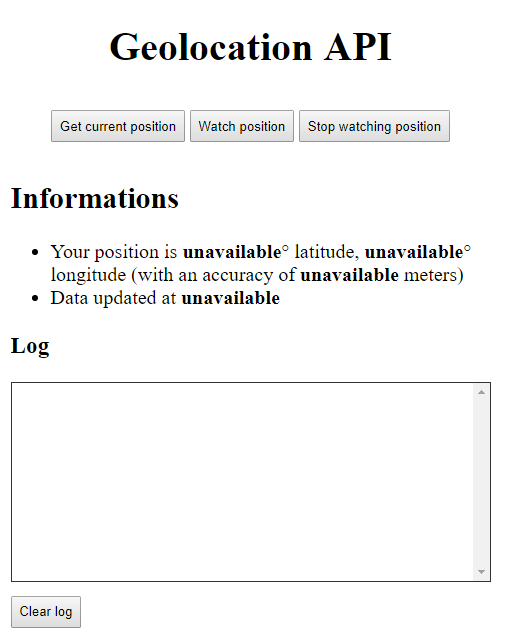
\includegraphics[width=0.5\linewidth]{geo1}
		\caption{Pagina info Geolocation}
		\label{fig: Pagina info Geolocation}
	\end{figure}
	\pagebreak
	\\
	Quando saranno chiamati i metodi \textit{getCurrentposition} o \textit{WatchPosition} verrà chiesto all'utente il permesso per usare la posizione.
	\begin{figure}[h]
		\centering
		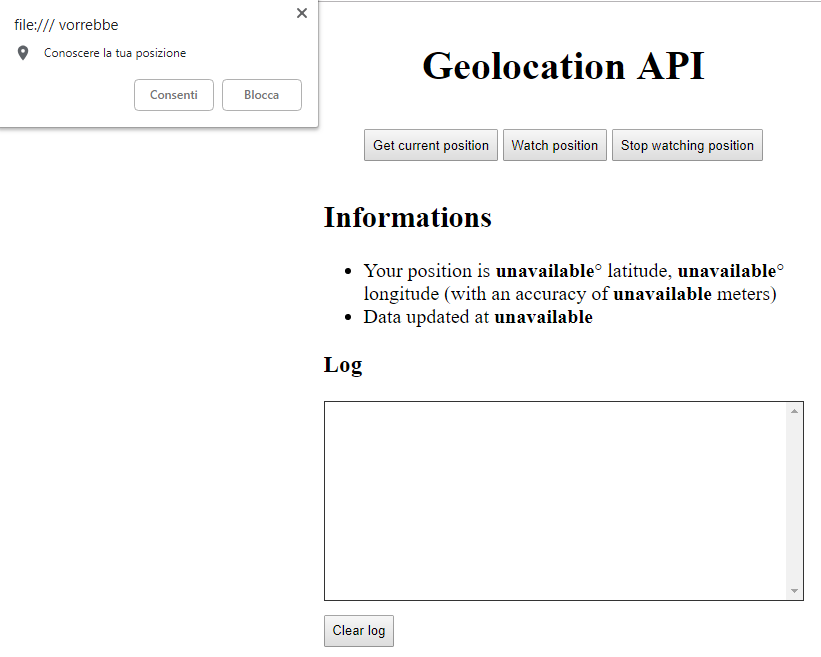
\includegraphics[width=0.4\linewidth]{geo2}
		\caption{Richiesta permesso}
		\label{fig: Richiesta permesso}
	\end{figure}
	\\
	Se l'utente rifiuta la posizione non viene calcolata e viene mostrato un messaggio di errore in console.
	\begin{figure}[h]
		\centering
		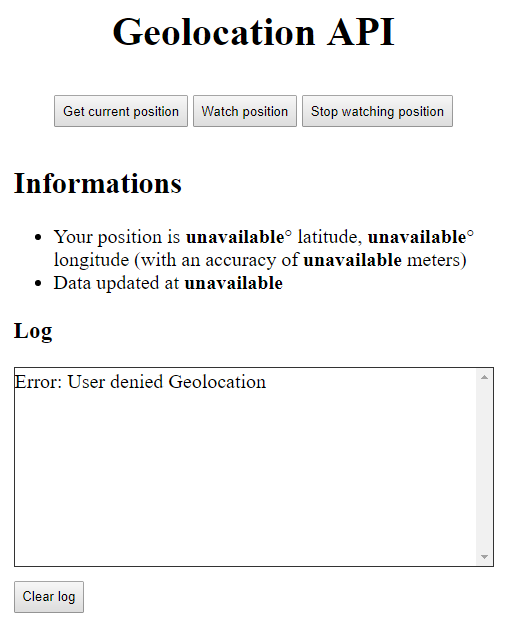
\includegraphics[width=0.4\linewidth]{geo3}
		\caption{Rifiuto autorizzazione}
		\label{fig: Rifiuto autorizzazione}
	\end{figure}
	\pagebreak
	\\
	Se l'utente acconsente all'utilizzo della posizione verrà mostrato un messaggio di conferma in console e saranno mostrate a video tutte le informazioni disponibili dell'utente.
	\begin{figure}[h]
		\centering
		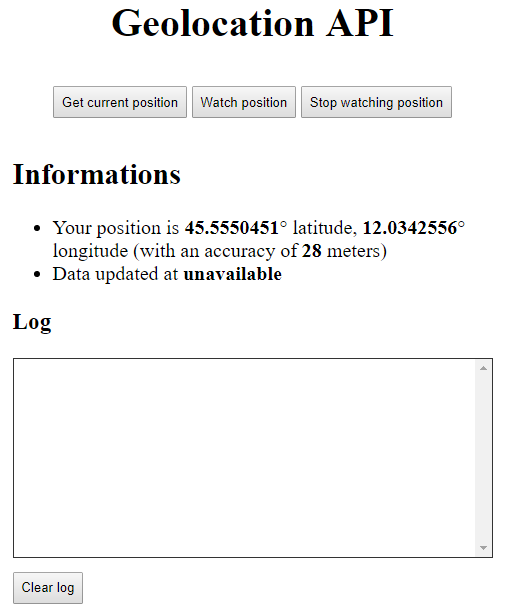
\includegraphics[width=0.4\linewidth]{geo4}
		\caption{Accetto autorizzazione}
		\label{fig: Accetto autorizzazione}
	\end{figure}
	\\
	
	
	\section{Rischi e sicurezza} 
	Uno dei principali problemi della Geolocation API \cite{rif6} \cite{rif7} è rappresentato dal fatto che un Web Attacker può rubare la posizione ad un utente che accetta di condividerla all'interno del sito attaccante ignaro del fatto che non sia sicuro, oppure attraverso un cross-site scripting (XSS) \footnote{Tipo di vulnerabilità di sicurezza presente nelle applicazioni web. Questo attacco consente agli aggressori di inserire script sul lato client in pagine Web visualizzate da altri utenti, e questa vulnerabilità può essere usata dagli aggressori per bypassare i controlli di accesso, come ad esempio la same origin policy.} all'interno di un sito considerato fidato. Gli oggetti per tracciare le coordinate (latitudine e longitudine) risiedono all'interno del DOM il quale è accessibile con JavaScript e attraverso il quale si possono prendere le informazioni sulla posizione dell'utente. 
	Nella maggior parte dei casi succede che la posizione viene richiesta e condivisa in quanto viene chiesta in siti web affidabili.
	Un problema importante è che se l'utente non disabilita il tracciamento della posizione il browser continuerà a esporla all'attaccante.
	\begin{figure}[h]
		\centering
		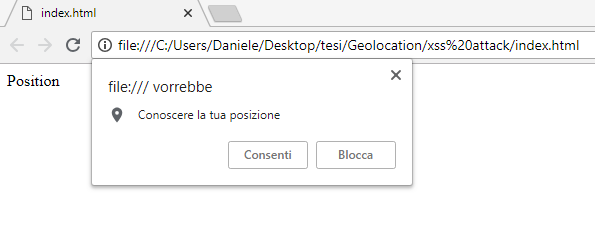
\includegraphics[width=0.5\linewidth]{pos1}
		\caption{Richiesta posizione}
		\label{fig: Richiesta posizione}
	\end{figure}
	\pagebreak
	\\
	Supponiamo che un utente malintenzionato abbia avuto modo di inserire una vulnerabilità XSS in un sito Web; tutto ciò che dovra fare è fare in modo che la vittima esegua il seguente codice JavaScript per rubare la posizione.
	\lstinputlisting{code/script.js}
	Il codice utilizza le proprietà del DOM \textit{cords.latitude} e \textit{cords.langitude} per determinare rispettivamente la latitudine e longitudine, memorizzandole in una variabile, inviandole poi all'attaccante. 
	\\
	\section{Compatibilità web}
	\subsection{Desktop e mobile}
	\begin{figure}[h]
		\centering
		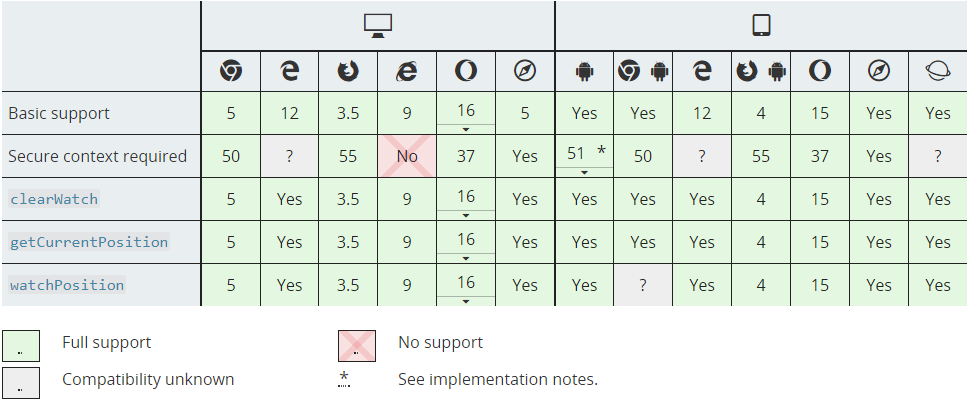
\includegraphics[width=1\linewidth]{compatibility}
		\caption{Compatibilità Desktop e mobile}
		\label{fig: Compatibilità Desktop e mobile}
	\end{figure}
	\section{Conclusioni}
	Abbiamo analizzato le specifiche e i problemi di privacy di una delle API più semplici del Web che, come ogni tecnologia, può essere un'arma a doppio taglio. 
	Tutti i threat model citati all'inizio della tesi possono essere identificati nel paragrafo.
	Come primo scenario consideriamo l'utente che usa l'API per migliorare l'esperienza utente: se guardiamo al commercio nel web, che negli ultimi anni ha preso sempre più piede, grazie alla geolocalizzazione gli utenti potranno avere sempre pubblicità mirata e personalizzata nei contenuti, della quale ne approfittano professionisti del marketing, rivenditori, enti governativi, forze dell'ordine, ecc; oppure possiamo considerare il fatto che grazie alla geolocalizzazione si possa ritrovare il proprio cellulare smarrito o rubato.
	Per passare al secondo threat model, ovvero un utente usa l'API ma non sa che ci possono essere conseguenze negative, possiamo prendere a titolo d'esempio un'azienda che, adottando tale tecnologia, potrebbe aumentare il rischio della privacy personale e dei dipendenti nel caso alcuni dati vengano rubati. 
	Considerando l'ultimo scenario, ovvero un attaccante che usa le API intenzionalmente in modo malevolo. Questa persona potrebbe avere le informazioni di un tag GPS e di geolocalizzazione, in combinazione con altre informazioni personali, e usarle per identificare il luogo presente o futuro di un individuo, facilitando la possibilità di causare danni a persone e/o proprietà (furto, stalking, rapimento, violenza domestica, furto d'identità, ecc). Ovviamente il crimine fisico è meno prevalente del crimine informatico attraverso il quale, tramite i dati di geolocalizzazione IP, si può identificare la posizione fisica del computer dell'utente dal quale si possono rubare informazioni personali (indirizzo di casa, lavoro, scuola, itinerari giornalieri, carte di credito, ecc). Chiaramente, come detto precedentemente, il fattore di rischio si estende non solo all'individuo ma anche a imprese, dipendenti e via dicendo.
	Inoltre, quando qualcuno utilizza un'applicazione, potrebbero esserci più servizi che controllano i dati: il fornitore di tali servizi, i punti di accesso, gli sviluppatori, ecc. e molte volte gli utenti non riescono a capire l'origine della raccolta di tali dati. 
	Questo fattore, assieme al modo in cui vengono utilizzati, con chi sono condivisi, se saranno traferiti altrove, per quanto saranno conservati e da chi, sollevano preoccupazioni agli utenti. 
	Chiaramente esistono diversi modi per mitigare questi rischi, ad esempio attraverso soluzioni di salvaguardia tecnologica e/o attraverso la consapevolezza dell'utente di tali rischi.
	\\
	Col passare del tempo ci saranno sempre nuove tecnologie e nuovi servizi, argomenti e temi ricorrenti che la società continuerà a considerare e discutere in positivo o negativo.
	Si potrebbe essere contenti di avere la vita semplificata per alcune tecnologie offerteci, come in questo caso per quanto riguarda la geolocalizzazione, ma al contempo si potrebbe essere preoccupati per la propria privacy: chi ha i miei dati? Come vengono usati? Sono protetti?
	\cleardoublepage
	
	\chapter{PaymentRequest API}
	
	\section{Overview}
	La PaymentRequest API \cite{rif9} nasce con l'intento di creare esperienze di pagamento semplificate, in quanto ogni sito web ha il proprio sistema di pagamento e molti siti richiedono la ridigitazione manuale delle stesse informazioni più volte, le quali possono essere invece memorizzate e riutilizzate dall'API per completare più rapidamente le transazioni online.
	
	\subsection[Vantaggi]{Vantaggi \cite{rif13}}
	\begin{itemize}
		\item \textbf{Esperienza di acquisto rapida:} gli utenti immettono i propri dati una sola volta nel browser, e dopo averli inseriti non è più necessario reinserirli su siti diversi;
		\item \textbf{Esperienza coerente su ogni sito che supporta l'API:} poiché la pagina di pagamento è controllata dal browser si può personalizzare l'esperienza utente, ad esempio includendo la localizzazione per impostare automaticamente la lingua preferita dell'utente o altre features;
		\item \textbf{Gestione delle informazioni:} gli utenti possono gestire le loro carte di credito e gli indirizzi di spedizione direttamente nel browser. Un browser può anche sincronizzare queste informazioni tra dispositivi, rendendo più semplice per gli utenti passare dal desktop al cellulare e viceversa quando si acquistano oggetti;
		\item \textbf{Gestione coerente degli errori:} il browser può controllare la validità dei numeri delle carte e può comunicare all'utente se una carta è scaduta o sta per scadere, può suggerire automaticamente quale carta utilizzare in base ai modelli di utilizzo passati o alle restrizioni del commerciante, o consentire all'utente di dire quale sia la carta predefinita/preferita;
		\item \textbf{Esperienza utente migliorata:} coerenza tra i siti Web, tra browser e sistemi operativi e nuove funzionalità del browser per semplificare il checkout, ecc;
		\item \textbf{Miglioramento della sicurezza:} la PaymentRequest API ha il potenziale per ridurre le opportunità di frode e può facilitare l'adozione di metodi di pagamento più sicuri. Purtroppo ci sono dei problemi di sicurezza analizzati al paragrafo 3.4; 
		\item \textbf{Responsabilità inferiore:} in passato, per creare un'esperienza utente semplificata, i commercianti dovevano memorizzare le credenziali di pagamento degli utenti. \\Questo non è più necessario, il che può aiutare a ridurre la responsabilità del commerciante nei confronti del cliente.
	\end{itemize}
	
	\subsection{Come funziona}	
	La PaymentRequest API consente a un utente di completare una transazione più facilmente riutilizzando le informazioni memorizzate nel browser o in app di pagamento di terze parti.
	Quando l'utente preme un pulsante in una pagina di checkout collegata all'API il commerciante utilizza l'API per richiedere il pagamento. Il commerciante fornisce informazioni su prezzo, valuta e un elenco di metodi di pagamento accettati, e può inoltre richiedere al browser di creare un'interfaccia utente semplificata per raccogliere l'indirizzo di spedizione, le informazioni di contatto e altri elementi all'utente.
	Il browser determina quali metodi di pagamento sono supportati dal commerciante tra le varie "app di pagamento" mostrandole all'utente. 
	L'utente seleziona un'app di pagamento con la quale pagare, la quale può comportare ulteriori interazioni con l'utente (ad esempio per l'autenticazione). 
	Al completamento l'app di pagamento restituisce i dati tramite l'API al commerciante.
	
	\begin{figure}[h]
		\centering
		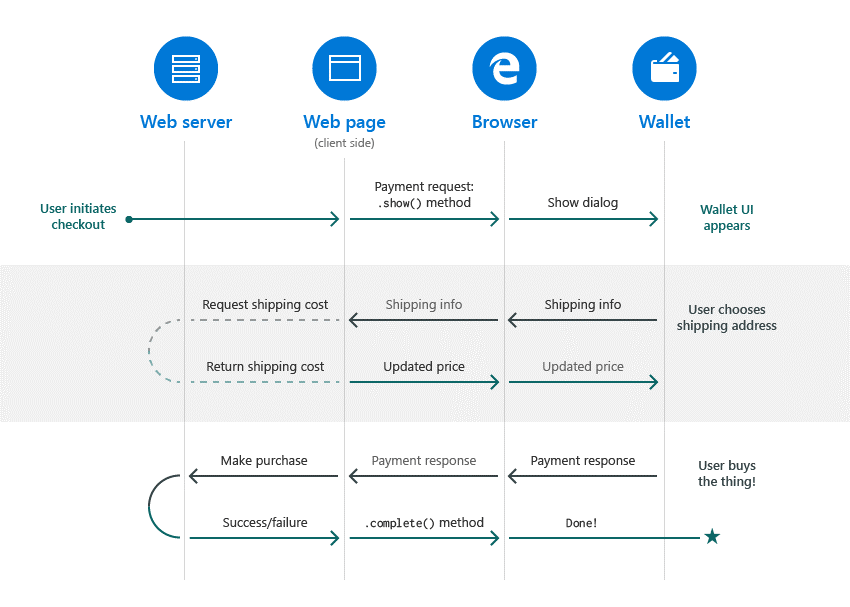
\includegraphics[width=1\linewidth]{SchemaPayment}
		\caption{Schema Payment Request API \cite{rif17}}
		\label{fig:Schema Payment}
	\end{figure}
	\pagebreak
	
	\subsection{Uso API}
	\textbf{Ruolo dell'utente}
	\\
	Gli utenti beneficiano del riutilizzo delle informazioni inserite nel browser o nelle app di pagamento. Quindi, quando si visita un sito Web che sfrutta la PaymentRequest API gli utenti avranno l'opportunità di sfruttare il riutilizzo semplificato delle informazioni archiviate.
	\\
	\textbf{Ruolo del commerciante}
	\\
	L'API influisce sul front end (l'interfaccia dell'esperienza utente) e non sul back-end, pertanto il commerciante non dovrebbe dover apportare modifiche all'elaborazione back-end dei vari metodi di pagamento; questo sarà compito del fornitore della pagina di pagamento il quale sostituirà i moduli Web con le chiamate alla PaymentRequest API.
	\\
	\textbf{Ruolo del browser}
	\\
	Il browser svolge diversi ruoli:
	\begin{itemize}
		\item Calcola l'intersezione dei metodi di pagamento accettati dal commerciante e registrati dall'utente;
		\item Visualizza l'interfaccia utente che consente all'utente di inserire le proprie informazioni;
		\item Funge da canale per i dati da e verso il commerciante e da e verso l'utente.
	\end{itemize}
	%\textbf{Metodi di pagamento}
	%\\
	%La PaymentRequest API è progettata per funzionare con un gran numero di metodi di pagamento, i quali vengono identificati attraverso due strade:
	%\begin{itemize}
	%	\item I metodi di pagamento definiti da W3C sono identificati come "basic-card" e sono composti da stringhe corte;
	%	\item I metodi di pagamento definiti da altre parti sono identificati dagli URL.
	%\end{itemize}
	\textbf{App di pagamento}
	\\
	La PaymentRequest API determina se un'app di pagamento "corrisponde" a una determinata transazione definendo un algoritmo che considera i metodi di pagamento accettati dal commerciante, dichiarati attraverso un elenco di identificativi del metodo di pagamento, passati attraverso l'API.
	Al fine di proteggere la privacy degli utenti i commercianti hanno accesso a informazioni molto limitate dell'utente. 
	
	Vediamo in che modo la PaymentRequest API influisce sul flusso dei metodi di pagamento che già supporta. Il normale flusso per gli utenti di solito implica qualcosa del genere:
	\begin{itemize}
		\item Scansione di un elenco di metodi di pagamento accettati;
		\item Scelta di un metodo;
		\item Per i metodi di pagamento che prevedono il lancio di un'app o la visita a un sito Web si invia l'utente a quell'app o sito;
		\item Pagamento completato.
	\end{itemize}
	La PaymentRequest API consente un flusso migliorato:
	\begin{itemize}
		\item L'utente preme un pulsante di acquisto singolo;
		\item Il browser visualizza le app di pagamento dell'utente che possono essere utilizzate per la transazione, ed è probabile che i browser supportino le preferenze dell'utente in modo che un'app di pagamento venga avviata automaticamente su un determinato sito Web, semplificando il checkout.
		\item Per i metodi di pagamento che prevedono il lancio di un'app o la visita a un sito Web, inviare l'utente a quell'app o sito; 
		\item Pagamento completato; 
	\end{itemize}
	\textbf{Differenze tra metodo di pagamento e app di pagamento}
	\\
	Un'app di pagamento è il software che l'utente utilizza per pagare, la quale può supportare uno o più metodi di pagamento e può essere implementata utilizzando diverse tecnologie. I browser possono anche fungere da app di pagamento, memorizzando le credenziali dell'utente. In generale più app di pagamento possono implementare lo stesso metodo di pagamento. 
	Vi sono casi importanti in cui è disponibile una sola app di pagamento autorizzata a supportare un metodo di pagamento, mentre ci sono casi in cui più app di pagamento possono servire diversi metodi di pagamento. In questo caso non è il commerciante che deve preoccuparsi dell'integrazione software, ma deve solamente richiedere le informazioni attraverso la PaymentRequest API.
	
	\section{Specifiche}
	\subsection[Metodi]{Metodi \cite{rif1}}
	Per utilizzare l'API lo sviluppatore deve fornire e tenere traccia di una serie di informazioni chiave, le quali vengono passate al costruttore PaymentRequest come argomenti e successivamente utilizzate per aggiornare la richiesta di pagamento visualizzata all'utente. Queste informazioni sono:
	\begin{itemize}
		\item \textbf{PaymentMethodData:} rappresenta i metodi di pagamento che il sito supporta;
		\item \textbf{PaymentDetails:} rappresenta i dettagli della transazione. Ciò include il costo totale e facoltativamente un elenco di beni o servizi acquistati, beni materiali, opzioni di spedizione o "modificatori" su come vengono effettuati i pagamenti: ad esempio "se paghi con una carta di credito di tipo X incorre in una tassa di elaborazione di tot";
		\item \textbf{PaymentOptions:} il PaymentOptions viene passato al costruttore PaymentRequest e fornisce informazioni sulla consegna del prodotto: ad esempio per i beni fisici il commerciante avrà bisogno di un indirizzo fisico dove spedire, mentre per i beni digitali e sufficeinte un'e-mail. Una volta che il PaymentRequest è stato costruito viene presentato all'utente finale tramite il metodo show(), il quale ritorna una promise che, una volta che l'utente conferma la richiesta di pagamento, si traduce in una PaymentResponse;
		\item \textbf{PaymentRequest:} la PaymentRequest serve a effettuare una richiesta di pagamento, in genere associata all'avvio di un processo di pagamento da parte dell'utente. La PaymentRequest consente agli sviluppatori di scambiare informazioni con l'user agent mentre l'utente sta fornendo dati in input. Poiché la visualizzazione simultanea di più interfacce PaymentRequest potrebbe confondere l'utente, questa specifica limita lo user agent a visualizzarne uno alla volta tramite il metodo show();
		\item \textbf{PaymentDetailsInit:} Il PaymentDetailsInit viene utilizzato nella costruzione della richiesta di pagamento;
		\item \textbf{PaymentResponse:} un PaymentResponse viene restituito quando un utente ha selezionato un metodo di pagamento e approvato una richiesta di pagamento.
	\end{itemize}
	
	\pagebreak
	\textbf{PaymentMethodData}
	\\
	\textit{PaymentMethodData} \cite{rif11} contiene gli identificativi dei metodi di pagamento accettati dal sito Web e qualsiasi dato specifico del metodo di pagamento associato.
	\lstinputlisting{code/PaymentMethodData.js}
	\textbf{PaymentDetails}
	\\
	I \textit{details} \cite{rif14} contengono informazioni sulla transazione che l'utente è invitato a completare.
	\lstinputlisting{code/PaymentDetails.js}
	\pagebreak
	\textbf{Opzioni di spedizione}
	\\
	Qui vediamo un esempio di come aggiungere due opzioni di spedizione ai \textit{details} \cite{rif16}.
	\lstinputlisting{code/OpzioniSpedizione.js}
	
	\flushleft\textbf{Modifiche condizionali alla richiesta di pagamento}
	\\
	Qui vediamo come aggiungere una tassa di elaborazione per l'utilizzo di una carta di credito. Si noti che richiede il ricalcolo del totale.
	\lstinputlisting{code/Tassa.js}
	\pagebreak
	\textbf{PaymentOptions} \\
	\textit{Options} contiene informazioni che lo sviluppatore ha bisogno dall'utente per eseguire il pagamento.
	\lstinputlisting{code/PaymentOptions.js}
	
	\textbf{PaymentRequest} \\
	Dopo aver raccolto tutti i bit di informazioni prerequisite, ora possiamo costruirne uno \textit{PaymentRequest} e richiedere che il browser lo presenti all'utente.
	\lstinputlisting{code/PaymentRequest.js}
	\pagebreak
	
	\subsection{Implementazione su pagina d'esempio}
	%rif15
	\subsubsection{Costruttore}
	L'oggetto \textit{PaymentRequest} è costruito passando i seguenti parametri:
	\begin{itemize}
		\item \textbf{methodData:} una serie di identificativi del metodo di pagamento e tutti i dati pertinenti. Un identificativo del metodo di pagamento è una stringa che identifica un metodo di pagamento supportato;
		\item \textbf{details:} contiene le informazioni sulla transazione, come gli elementi pubblicitari in un ordine;
		\item \textbf{options:} contiene informazioni aggiuntive che il Wallet potrebbe dover raccogliere.
	\end{itemize}
	
	Nel seguente esempio stiamo consentendo agli utenti di pagare con qualsiasi carta di debito o di credito appartenente alle reti Visa, MasterCard o Amex. L'oggetto \textit{details} contiene l'importo totale parziale, l'imposta sulle vendite e il totale dovuto; questi dettagli verranno mostrati all'utente nel portafoglio. Bisogna tenere presente che l'API non aggiunge elementi o calcola l'imposta sulle vendite, spetta al commerciante fornire le informazioni corrette. In questo esempio, stiamo vendendo un bene fisico, quindi chiediamo l'indirizzo di spedizione del cliente.
	\lstinputlisting{code/Costruttore.js}
	\subsubsection{Visualizzazione dell'interfaccia utente, elaborazione del pagamento e visualizzazione dei risultati}
	Una volta creato l'oggetto \textit{PaymentRequest} è possibile attivare il browser per visualizzare il wallet con \textit{request.show()} \cite{rif2}. 
	\begin{figure}[h]
		\centering
		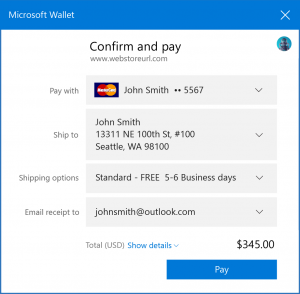
\includegraphics[width=0.5\linewidth]{wallet1}
		\caption{Wallet dopo la chiamata request.show()}
		\label{fig: Wallet dopo la chiamata request.show()}
	\end{figure}
	\\
	
	I clienti possono  selezionare le informazioni di pagamento, l'indirizzo di spedizione e altri campi appropriati e cliccare su Paga quando è pronto. A questo punto, gli utenti dovranno verificare la loro identità: in caso di esito positivo verrà soddisfatta la promise \textit{request.show()} e verranno restituite al sito Web tutte le informazioni che il cliente ha fornito. Per il metodo di pagamento con carta di base l'oggetto risultante conterrà il nome del titolare della carta, il numero della carta, il mese di scadenza e altri campi pertinenti. Il commerciante può quindi utilizzare queste informazioni per elaborare la transazione sul back-end.
	Dopo che la risposta è tornata dal server, è possibile utilizzare \textit{result.complete('success')} per visualizzare la schermata di successo o \textit{result.complete('fail')} per indicare una transazione fallita.
	\lstinputlisting{code/PaymentShow.js}
	\pagebreak
	Ed ecco i wallet in caso di successo e di fallimento.
	\begin{figure}[h]
		\centering
		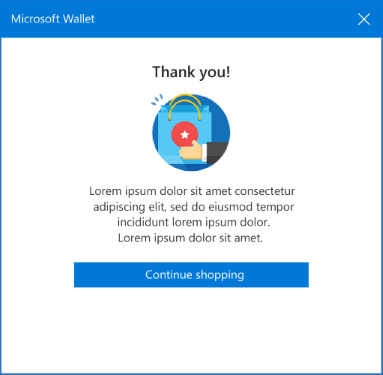
\includegraphics[width=0.5\linewidth]{wallet2}
		\caption{Wallet in caso di successo}
		\label{fig: Wallet in caso di successo}
	\end{figure}
	\begin{figure}[h]
		\centering
		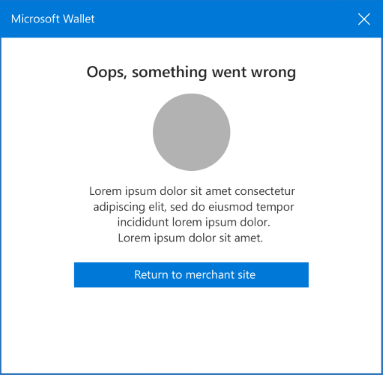
\includegraphics[width=0.5\linewidth]{wallet3}
		\caption{Wallet in caso di fail}
		\label{fig: Wallet in caso di fail}
	\end{figure}
	\pagebreak
	
	\section[Rischi e sicurezza]{Rischi e sicurezza \cite{rif19}} 
	La PaymentRequest API cerca di garantire la sicurezza dei dati sensibili nei seguenti modi:
	
	\begin{itemize}
		\item Per garantire che gli utenti non condividano inavvertitamente informazioni sensibili con una certa origine, l'API richiede che il proprio metodo \textit{show()} venga attivato solo tramite la volontà da parte dell'utente, ad esempio con un clic. Inoltre, per evitare un'esperienza utente confusa, questa specifica limita la visualizzazione di una finestra alla volta del metodo \textit{show()} così da non rischiare di inserire dati in più pagine, le quali potrebbero risultare untrusted. 
		Se infatti si prova ad aprire più di una finestra dell'API accadrà la seguente situazione:
		
		\begin{figure}[h]
			\centering
			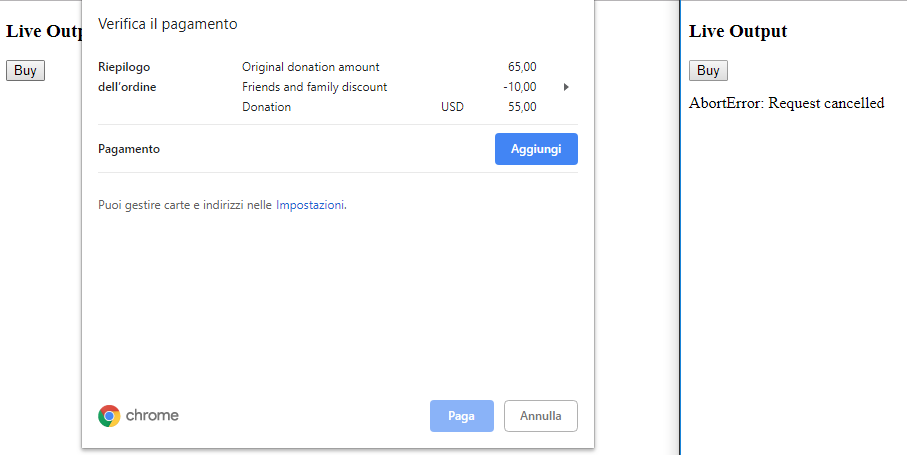
\includegraphics[width=0.5\linewidth]{Buy}
			\caption{Metodo show() richiamato più volte}
			\label{fig: Metodo show() richiamato più volte}
		\end{figure}
		
		
		\item La PaymentRequest API è disponibile solamente su HTTPS, quindi lavora solamente in contesti sicuri per aumentare la sicurezza dell'inserimento delle informazioni. 
		
		\item I commercianti possono delegare la memorizzazione delle informazioni ai fornitori di servizi di pagamento o al browser, senza avere l'onere di memorizzare le informazioni sensibili dell'utente. Inoltre, ovviamente, le informazioni dell'utente non devono essere condivise con uno sviluppatore senza l'autorizzazione dell'utente.
	\end{itemize}
	
	Purtroppo un possibile rischio potrebbe essere quello di essere vittima di phishing nel caso fossimo in una pagina untrusted, ovvero viene aperta una pagina identica a quella in cui siamo e tutte le credenziali che inseriamo vengono mandate all'attaccante invece che al sito dove pensiamo di essere. 
	Un altro possibile rischio invece potrebbe essere quello di essere vittima di un attacco XSS, ovvero un tipo di attacco nel quale degli script dannosi vengono inseriti lato server all'interno di siti affidabili, dove l'utente è ignaro di questo (questo tipo di attacco verrà spiegato nel prossimo paragrafo).
	
	Chiaramente esistono diversi modi per mitigare questi rischi, ad esempio attraverso soluzioni di salvaguardia tecnologica e/o attraverso la consapevolezza dell'utente di tali rischi.
	
	\subsection[Esempio di un possibile attacco]{Esempio di un possibile attacco \cite{rif18}} 
	\textbf{Descrizione dell'attacco}
	\\
	Supponiamo di essere all'interno di un sito affidabile, come Amazon o Facebook, e supponiamo di essere in una pagina di pagamento, come può essere il carrello su Amazon o il pagamento per un'inserzione su Facebook.
	Se un attaccante riesce a inserire degli script all'interno di queste pagine riuscirà a ribare le informazioni di pagamento di un utente.
	Quando l'utente cliccherà sulla voce "paga", in una delle due piattaforme le quali sono considerate affidabili, verrà eseguito lo script malevolo, invece di quello trusted del sito.
	L'utente inserirà tutte le informazioni necessarie al pagamento ma queste verranno mandate e/o visualizzate dall'attaccante.
	Come mostrato nell'esempio in figura 14 in questo modo tutte le informazioni possono essere visualizzate dall'attaccante.
	Alla richiesta di avvio di un processo di pagamento, ovvero dopo la chiamata al metodo \textit{show()}, viene creato l'oggetto PaymentRequest nel quale vengono inseriti tutti i dati che l'utente inserisce. 
	\begin{figure}[h]
		\centering
		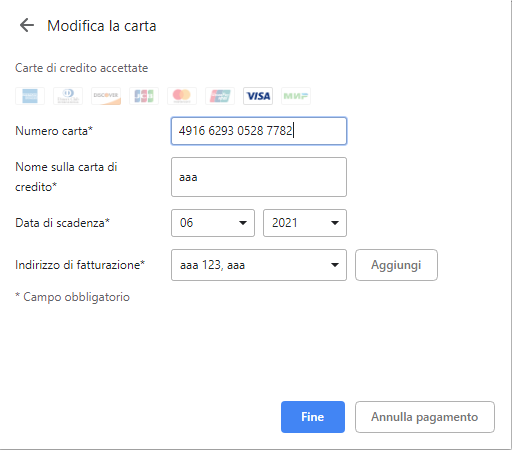
\includegraphics[width=0.5\linewidth]{Chrome1}
		\caption{Inserimento informazioni dell'utente}
		\label{fig: Inserimento informazioni dell'utente}
	\end{figure}
	\\
	Una volta che l'utente ha approvato una richiesta di pagamento viene restituito un \textit{PaymentResponse} per approvare tale richiesta. 
	\begin{figure}[h]
		\centering
		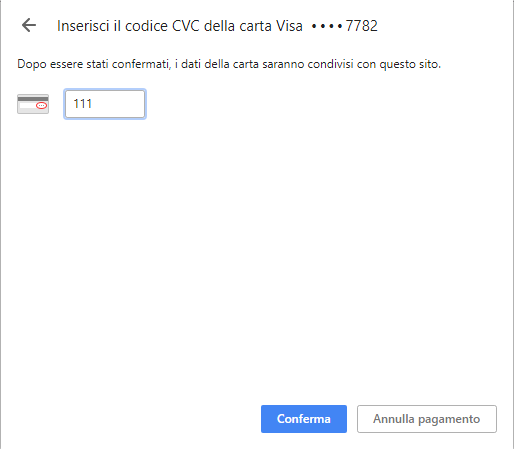
\includegraphics[width=0.5\linewidth]{Chrome2}
		\caption{Inserimento CVV}
		\label{fig: Inserimento CVV}
	\end{figure}
	\\
	\pagebreak
	L'oggetto \textit{PaymentRequest}, creato in precedenza e contenente i dati dell'utente, passa però attraverso il DOM, e quindi può essere intercettato e può essere visualizzato ogni campo inserito dall'utente. Ad esempio nel campo \textit{details.cardNumber} si può leggere il numero di carta di credito, mentre in \textit{details.cardSecurityCode} si può leggere il codice CVV; entrambi sono mostrati nell'esempio nella figura seguente.
	\begin{figure}[h]
		\centering
		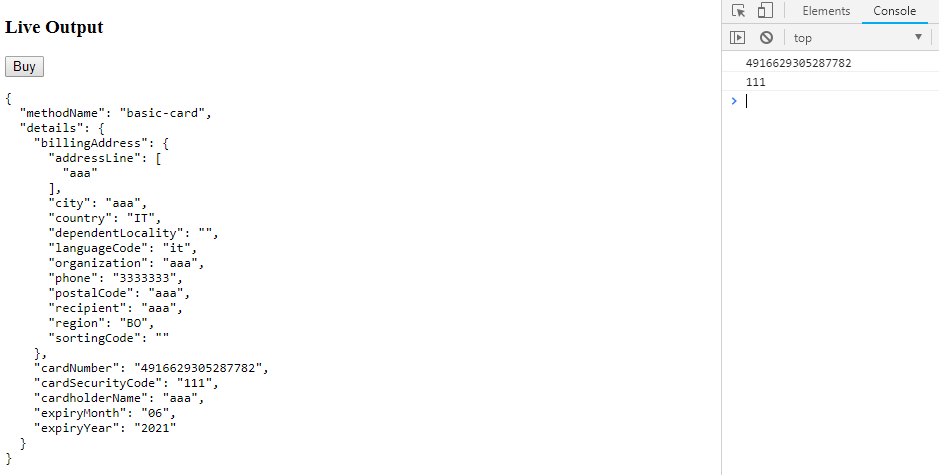
\includegraphics[width=1\linewidth]{Informazioni}
		\caption{Informazioni rubate}
		\label{fig: Informazioni rubate}
	\end{figure}
	\section{Compatibilità web}
	\subsection{Desktop}
	\begin{figure}[h]
		\centering
		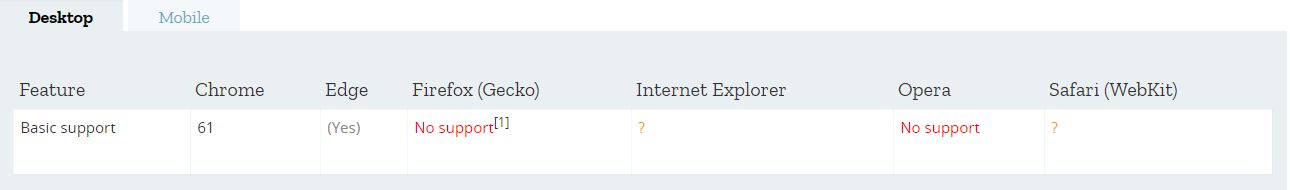
\includegraphics[width=1\linewidth]{Compatibilita1}
		\caption{Compatibilità desktop}
		\label{fig: Compatibilità desktop}
	\end{figure}
	\subsection{Mobile}
	\begin{figure}[h]
		\centering
		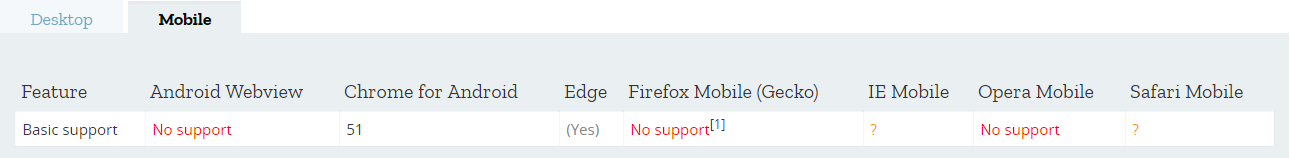
\includegraphics[width=1\linewidth]{Compatibilita2}
		\caption{Compatibilità mobile}
		\label{fig: Compatibilità mobile}
	\end{figure}
	\section{Conclusioni}
	La PaymentRequest API è uno strumento per migliorare l'esperienza utente sul Web offrendo ai clienti un'esperienza di acquisto più piacevole ma, come ogni strumento informatico, ha delle vulnerabilità.
	Come nel paragrafo precedente, anche qui abbiamo analizzato le specifiche e i problemi di privacy che tale API può avere e, come prima, identificheremo i vari threat model.
	Per quanto riguarda il migliorare l'esperienza utente abbiamo visto come questa API semplifichi notevolmente le esperienze di pagamento memorizzando le informazioni e riutilizzandole per completare in maniera più veloce le transazioni online. 
	Considerando il secondo threat model, dove un utente usa l'API a fin di bene non sapendo però dell'esistenza del rischio, possiamo nominare due situazioni scritte nel capitolo 3.4: il phishing e l'attacco XSS.
	Prendendo in esame l'ultimo scenario, ovvero un attaccante che usa le API intenzionalmente in modo malevolo, si rimanda al paragrafo 3.4.1, dove vengono rubate le informazioni sensibili di un utente usando l'API ritenuta affidabile; questo di solito avviene nei siti non sicuri o, come detto prima, attraverso il phishing o gli attacchi XSS.
	I comportamenti per mitigare i rischi sono gli stessi della geolocation API, ovvero usare software di salvaguardia e/o avere consapevolezza di tali rischi all'interno del web.
	\newpage
	
	\cleardoublepage
	\chapter{Service Worker}
	\section{Overview}
	Un Service Worker \cite{rif23} \cite{rif24} \cite{rif25} è uno script Javascript che utilizza le \textit{Promises} \cite{rif27} per poter eseguire operazioni in modalità asincrona nel browser, avviate in background separato dalla pagina; pertanto non possono modificarne gli elementi del DOM come i normali script ma può comunicare con essi mediante “messaggi”.
	Un Service Worker si trova tra la nostra applicazione Web e la rete e, come un server proxy, può intercettare tutte le richieste a pagine web e file statici e rispondere secondo politiche che siamo noi stessi a decidere.
	I Service Worker sono pensati per consentire la creazione di esperienze offline efficaci \cite{rif28}, intercettare le richieste di rete e intraprendere azioni appropriate in base al fatto che la rete sia disponibile o meno e aggiornare le risorse che risiedono sul server, oltre a consentire l'accesso alle notifiche push e alle API di sincronizzazione in background.
	È il browser che in qualsiasi momento deciderà se il Service Worker dovrebbe essere o meno in esecuzione così da risparmiare risorse, specialmente sui dispositivi mobili. Per questo può essere che se non facciamo alcuna richiesta HTTP per un certo periodo di tempo o non riceviamo alcuna notifica per un po' è possibile che il browser spenga il Service Worker. Se attiviamo una richiesta HTTP che deve essere gestita dal Service Worker il browser la attiverà di nuovo, nel caso in cui non fosse ancora in esecuzione. 
	
	\subsection[Impostare i Service Worker]{Impostare i Service Worker \cite{rif22}}
	Molte funzionalità dei Service Worker oggi sono abilitate di default, ma nel caso non lo fossero bisogna abilitarle nel browser:
	\begin{itemize}
		\item Firefox: su \url{about:config} impostare \textit{dom.serviceWorkers.enabled} su true, riavvia il browser;
		\item Chrome : su \url{chrome://flags} accendere  \textit{experimental-web-platform-features}, riavvia browser;
		\item Opera : su \url{opera://flags} attivare \textit{Support for Service Worker}, riavvia il browser;
		\item Microsoft Edge : su \url{about:flags} spuntare  \textit{Enable Service Workers}, riavvia il browser.
	\end{itemize}
	
	\subsection{Architettura di base}
	Per quanto riguarda i Service Worker generalmente vengono eseguiti questi passaggi per l'impostazione di base:
	\begin{itemize}
		\item L'URL del Service Worker viene recuperato e registrato tramite \textit{serviceWorkerContainer.register()};
		\item In caso di esito positivo il Service Worker viene eseguito in un \textit{ServiceWorkerGlobalScope}, ovvero un tipo speciale di ServiceContext che scappa dal thread di esecuzione dello script principale senza accesso DOM. Il Service Worker ora è pronto per elaborare gli eventi;
		\item L'installazione del Service Worker viene tentata quando si accede successivamente alle pagine: un evento di installazione è sempre il primo inviato a un Service Worker;
		\item Quando il Service Worker è considerato installato il passo successivo è l'attivazione, quindi quando il Service Worker è installato riceve un evento di attivazione.
	\end{itemize}
	\begin{figure}[h]
		\centering
		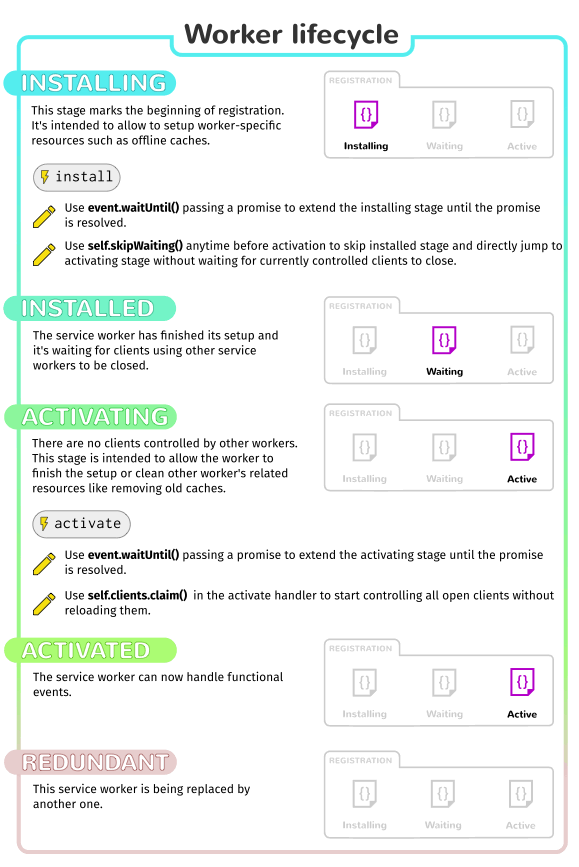
\includegraphics[width=0.6\linewidth]{SwLifecycle}
		\caption{Ciclo di vita del Service Worker}
		\label{fig:Ciclo di vita del Service Worker}
	\end{figure}
	
	\subsection{Casi d'uso}
	I Service Worker sono destinati anche ad altri usi:
	\begin{itemize}
		\item Sincronizzazione dei dati in background: viene avviato un Service Worker anche quando nessun utente si trova sul sito, quindi le cache possono essere aggiornate, ecc;
		\item Risposta a richieste di risorse da altre origini;
		\item Caching;
		\item Miglioramenti delle prestazioni, ad esempio prelettura delle risorse che l'utente probabilmente avrà bisogno nel prossimo futuro.
		\item Reagire per inviare messaggi: si può avviare un Service Worker per inviare agli utenti un messaggio per comunicare loro che sono disponibili nuovi contenuti;
		\item Reagendo ad orari e date particolari.
	\end{itemize}
	
	\section{Ciclo di vita di un Service Worker}
	Il ciclo di vita di un Service Worker \cite{rif20} \cite{rif21} \cite{rif26} è composto da quattro fasi:
	\begin{itemize}
		\item \textbf{Registrazione}: il Service Worker viene scaricato dal browser, analizzato ed eseguito;
		\item \textbf{Installazione}: il Service Worker viene installato;
		\item \textbf{Attivazione}: il Service Worker è pronto ed è in grado di poter controllare gli eventi generati dal client;
		\item\textbf{ Fetch}: evento generato dal client. Il Service Worker è in grado di intercettare le richieste e rispondere secondo le opportune strategie di caching. 
	\end{itemize}
	
	\subsection{Registrazione}
	
	Come prima cosa bisogna comunicare al browser l’esistenza di un ServiceWorker all’interno del sito web. Un Service Worker viene prima registrato utilizzando il metodo \textit{ServiceWorker.register()} e per farlo basta inserire su tutte le pagine del sito uno script come il seguente:
	\lstinputlisting{code/Registrazione.js}
	Il codice inizia controllando il supporto da parte del browser verificando la presenza di \textit{navigator.serviceWorker}. Se supportato, il Service Worker viene registrato per mezzo di \textit{navigator.serviceWorker.register} che restituisce un oggetto \textit{Promise} il quale si risolve con successo a registrazione avvenuta correttamente.
	\textit{service-worker.js} è il file Javascript residente nella root del sito web e che contiene il codice del Service Worker, il cui codice è:
	\pagebreak
	\lstinputlisting{code/Registrazione2.js}
	In questo modo viene registrato un Service Worker il quale viene semplicemente installato e ad ogni richiesta stampa in console un messaggio con la URL che il browser tenta di scaricare dal server web. Per controllare il caricamento di un Service Worker il codice di questo deve essere eseguito al di fuori delle normali pagine.
	
	Possono esserci diversi motivi per cui il Service Worker non si registra:
	\begin{itemize}
		\item Non si sta eseguendo l'applicazione tramite HTTPS;
		\item Il path del Service Worker non è scritto correttamente: deve essere scritto in relazione all'origine, non alla directory radice dell'app;
		\item Il Service Worker a cui ci si riferisce ha un'origine diversa da quella dell'app.
	\end{itemize}
	
	\subsection{Installazione}
	Il Service Worker viene scaricato immediatamente quando un utente accede per la prima volta a un sito, o una pagina, controllata dal Service Worker, e sarà poi scaricato periodicamente ogni tot periodo di tempo.
	
	L'installazione viene tentata quando il file nuovo che è stato scaricato risulta diverso da un Service Worker esistente, o risulta essere diverso dal primo Service Worker rilevato per quella pagina/sito. Se è la prima volta che un Service Worker viene reso disponibile viene tentata l'installazione e, dopo un'installazione corretta, viene attivato. Se è disponibile un Service Worker esistente la nuova versione viene installata in background, ma non ancora attivata; si attiva solo quando non ci sono più pagine caricate che stanno ancora utilizzando il vecchio Service Worker. Non appena non ci sono più pagine da caricare il nuovo Service Worker si attiva.
	
	Conseguentemente all’installazione viene richiamato l’evento \textit{install}: tale evento consente di effettuare il precaching, ovvero inserire in cache pagine e file statici del sito web prima di intercettarne le richieste. Per farlo occorre utilizzare gli oggetti \textit{Promise} e cache come segue:
	\pagebreak
	\lstinputlisting{code/Installazione.js}
	Se si decidesse di aggiungere/eliminare nuove risorse da inserire in cache bisognerà avere l’accortezza di cambiare il nome della versione del Service Worker ed eliminare dalla cache le risorse già presenti.
	Una cosa molto importante da sapere è che le risorse da inserire in cache in fase di precaching devono esistere realmente sul server web altrimenti il Service Worker genererà un errore fatale e l’installazione non andrà a buon fine. 
	Il metodo \textit{skipWaiting()} consente al Service Worker di passare allo stato di attivazione ad installazione conclusa e quindi essere subito operativo.
	
	\subsection{Attivazione}
	Una volta installato il Service Worker passa nello stato di attivazione. Se la pagina al momento è controllata da un altro Service Worker quello attuale passa in uno stato di attesa per poi diventare operativo al prossimo caricamento di pagina quando il vecchio Service Worker viene sostituito.
	Questo per essere sicuri che solo un Service Worker (o una sola versione di Service Worker) per volta possa essere eseguito nello stesso contesto.
	A Service Worker attivato viene richiamato l’evento activate, ovvero l'evento per svuotare la cache obsoleta dell’eventuale precedente versione di Service Worker. Dopodiché il Service Worker sarà in grado di effettuare il fetching di risorse o di restare in attesa di altri eventi.
	Di default il nuovo Service Worker diventa operativo al refresh della pagina o dopo aver richiamato il metodo \textit{clients.claim()}; fino a quel momento le eventuali richieste non saranno intercettate. 
	
	\subsection{Fetch}
	Grazie all’evento fetch il Service Worker potrà agire da proxy tra l’applicazione web e la rete.
	Il Service Worker intercetterà ogni richiesta HTTP del browser e sarà in grado di rispondere a quest’ultimo prendendo la risorsa dalla cache piuttosto che scaricarla dalla rete.
	Grazie all’evento fetch il Service Worker diventa un vero e proprio strumento per migliorare le performance di caricamento di un sito web.
	
	\subsection{Aggiornare il Service Worker}
	Se il Service Worker è già stato installato ma una nuova versione è disponibile per l'aggiornamento o il caricamento della pagina, la nuova versione viene installata in background ma non sarà ancora attivata. Si attiva solo quando non ci sono più pagine caricate che stanno ancora utilizzando il vecchio servizio. Non appena non ci sono più pagine di questo tipo ancora caricate, il nuovo Service Worker si attiverà.
	
	Si dovrà aggiornare il listener install di eventi nel nuovo Service Worker, similmente a questo:
	\lstinputlisting{code/Aggiornamento.js}
	Mentre accade questo è ancora la versione precedente (v1) quella responsabile per i recuperi, mentre la nuova versione (v2) si sta installando in background.
	Quando nessuna pagina sta utilizzando la versione corrente, il nuovo operatore si attiva e diventa responsabile dei recuperi.
	
	\subsection{Disintallare il Service Worker}
	
	Rimuovere/disinstallare un Service Worker è un’operazione semplice. È possibile eseguirla manualmente dal proprio browser oppure inserendo un semplice script al posto di quello di registrazione del Service Worker:
	\lstinputlisting{code/Disinstallare.js}
	Naturalmente è necessario che la pagina contenente il codice di disinstallazione venga visitata dal browser, oppure è possibile rimuovere il Service Worker manualmente tramite DevTools.
	\newpage
	\section{Caching}
	Diverse sono le strategie che possono essere adottate per migliorare le performance di un sito web mediante i Service Worker. A seconda del sito e del contesto è possibile adottare una strategia piuttosto che l’altra:
	\begin{itemize}
		\item \textbf{Network first} \\
		Questa strategia mira ad avere un contenuto sempre fresco scaricandolo dalla rete, fornendo la copia in cache solo in caso di problemi di connettività, ad esempio in caso di connessione offline;
		\item \textbf{Cache first} \\
		Questa strategia verifica se la risorsa è disponibile in cache: se così fosse viene restituita la copia in cache, in caso contrario la risorsa viene scaricata dalla rete;
		\item \textbf{Network only} \\
		Viene simulato il normale comportamento del browser, ovvero scaricare le risorse direttamente dalla rete;
		\item \textbf{Cache only} \\
		In questo caso il Service Worker risponde solo con elementi conservati in cache: in caso di miss la risposta restituita al browser simulerà l’errore di connessione;
		\item \textbf{Fastest} \\
		Questa strategia mira a fornire all’utente la risposta più veloce: il Service Worker avvia contemporaneamente una richiesta in cache ed una in rete e la prima che risponde verrà restituita all’utente.
		Questa soluzione può essere l’ideale per quei dispositivi con vecchi hard drive dove la lettura da disco può  rivelarsi più lenta del fetch dalla rete, mentre per i dispositivi moderni è meglio utilizzare la strategia cache then network.
		\item \textbf{Cache then network} \\
		Questa strategia mira a fornire il contenuto dalla cache per una risposta molto rapida avviando una richiesta in rete scaricando una copia aggiornata della risorsa e sostituendola con quella in cache; la risorsa ricevuta dalla rete viene poi sostituita con quella presente sulla pagina.
	\end{itemize}
	È importante sottolineare che il Service Worker non utilizza cache a meno che non siamo noi a dirlo, quindi di default il comportamento nella fase di fetch delle risorse sarà quello nativo del browser.
	
	\begin{comment}
	Di seguito l’elenco completo delle strategie con esempi di codice di implementazione. 
	\subsubsection{Network first}
	Questa strategia mira ad avere un contenuto sempre fresco scaricandolo dalla rete, fornendo la copia in cache solo in caso di problemi di connettività (ad esempio in caso di connessione offline).
	\lstinputlisting{code/Networkfirst1.js}
	Una modifica interessante in questo caso potrebbe essere quella di aggiornare la copia in cache quando la risorsa viene scaricata dalla rete, cosicché in caso di errori di connessione viene restituita la copia più giovane.
	\lstinputlisting{code/Networkfirst2.js}
	\begin{figure}[h]
	\centering
	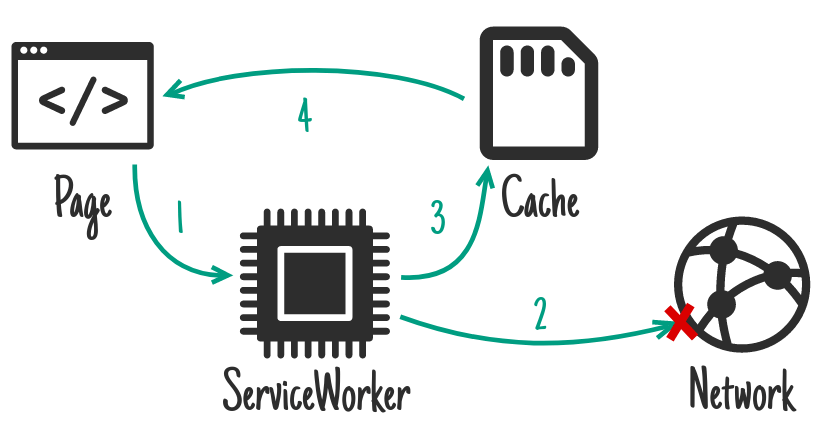
\includegraphics[width=0.7\linewidth]{Strategia1}
	\caption{Network first}
	\label{fig: Network first}
	\end{figure}
	\subsubsection{Cache first}
	Chiamata anche cache, falling back to network, questa strategia verifica se la risorsa è disponibile in cache. Se così fosse viene restituita la copia in cache. In caso contrario la risorsa viene scaricata dalla rete.
	\lstinputlisting{code/CacheFirst.js}
	\begin{figure}[h]
	\centering
	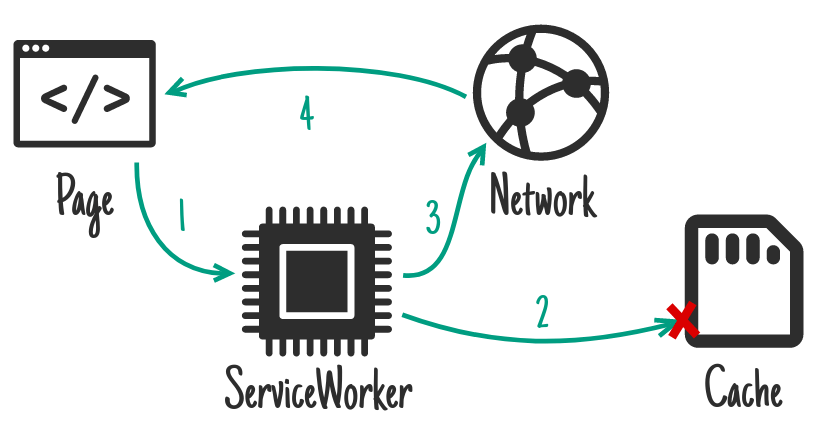
\includegraphics[width=0.7\linewidth]{Strategia2}
	\caption{Cache First}
	\label{fig: Cache First}
	\end{figure}
	\subsubsection{Network only}
	È la strategia più banale in quanto viene simulato il normale comportamento del browser, ovvero scaricare le risorse direttamente dalla rete.
	
	Per applicare  questa strategia basta non inserire alcuna riga di codice all’interno dell’evento fetch:
	\lstinputlisting{code/NetworkOnly1.js}
	o al limite inserire semplicemente la seguente riga:
	\lstinputlisting{code/NetworkOnly2.js}
	\begin{figure}[h]
	\centering
	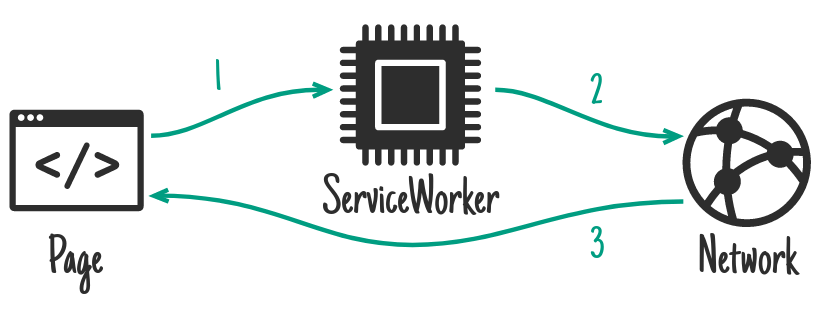
\includegraphics[width=0.7\linewidth]{Strategia3}
	\caption{Network only}
	\label{fig: Network only}
	\end{figure}
	\pagebreak
	\subsubsection{Cache only}
	Esattamente opposta alla strategia network only, in questo caso il Service Worker risponde solo con elementi conservati in cache. In caso di miss la risposta restituita al browser simulerà l’errore di connessione.
	\lstinputlisting{code/CacheOnly.js}
	\begin{figure}[h]
	\centering
	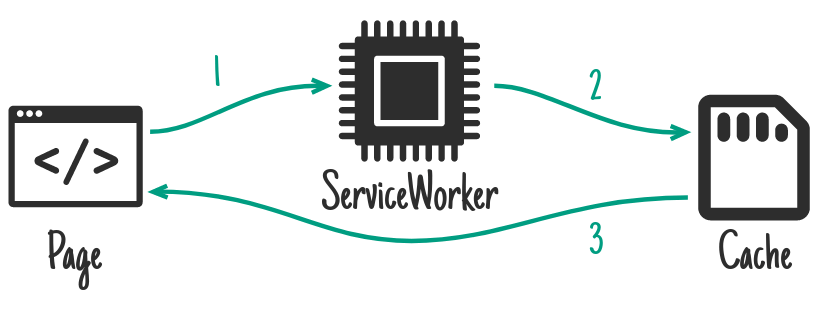
\includegraphics[width=0.7\linewidth]{Strategia4}
	\caption{Cache Only}
	\label{fig: Cache Only}
	\end{figure}
	\subsubsection{Fastest}
	Questa strategia mira a fornire all’utente la risposta più veloce. Il Service Worker avvia contemporaneamente una richiesta in cache ed una in rete. La prima che risponde verrà restituita all’utente.
	Questa soluzione può essere l’ideale per quei dispositivi con vecchi hard drive dove la lettura da disco può addirittura rivelarsi più lenta del fetch dalla rete. Per i dispositivi moderni è meglio utilizzare la strategia cache then network.
	Siccome il Service Worker può ritornare un solo Promise, occorre realizzare una funzione a cui passare un array di oggetti Promise, in questo caso cache e fetch, e risolverli quasi contemporaneamente ritornando quello che si risolve per primo.
	\pagebreak
	\lstinputlisting{code/Fastest.js}
	\begin{figure}[h]
	\centering
	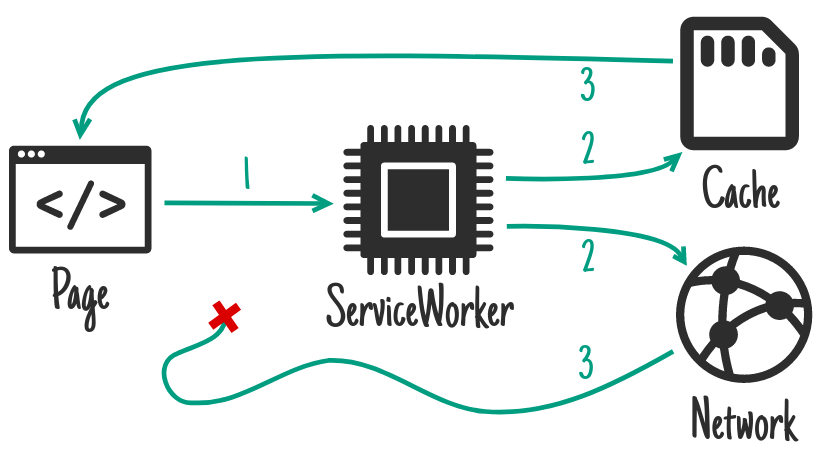
\includegraphics[width=0.7\linewidth]{Strategia5}
	\caption{Fastest}
	\label{fig: Fastest}
	\end{figure}
	\subsubsection{Cache then network}
	Questa strategia mira a fornire il contenuto dalla cache per una risposta molto rapida. Dopodiché in parallelo si avvia una richiesta in rete per scaricare una copia aggiornata della risorsa e sostituirla con quella in cache. La risorsa ricevuta dalla rete viene poi sostituita con quella presente sulla pagina.
	Per ottenere questo obiettivo occorre avere sia codice lato pagina che lato Service Worker. Questo perché il Service Worker deve rispondere subito e non può attendere il completamento di un secondo task senza rallentare l’intera operazione.
	Per ottenere qualcosa di analogo usando il solo Service Worker occorre utilizzare postMessage affinché la pagina comunichi al Service Worker la risorsa da interpellare con un secondo fetch, sia esso dalla cache o dalla rete. La complessità rimane uguale ma molto utile in caso si utilizzi il Service Worker per fare page caching.
	\begin{figure}[h]
	\centering
	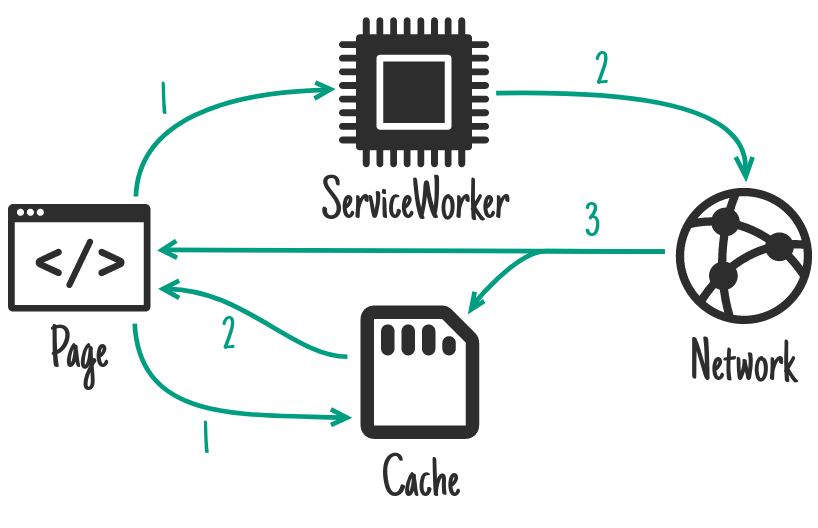
\includegraphics[width=0.7\linewidth]{Strategia6}
	\caption{Cache then Network}
	\label{fig: Cache then Network}
	\end{figure}
	\end{comment}
	\newpage
	\section[Rischi e sicurezza]{Rischi e sicurezza \cite{rif29}\footnote{\url{https://alf.nu/ServiceWorker}}}
	Come già detto i Service Worker operano solo in contesti protetti, ma questo non vuol dire che l'ambiente sia sicuro al 100\% in quanto un Service Worker ha la possibilità di importare script da qualsiasi altra origine tramite la chiamata a \textit{importScripts}, aumentando la capacità di un attaccante XSS di inserire il proprio codice javascript all'interno della pagina, potendo cosi rubare informazioni dell'utente, ad esempio all'inserimento di username e password in una data pagina, e portarle fuori. La registrazione dei Service Worker specifica che essi devono essere eseguiti nella stessa origine dei loro chiamanti; il confronto dell'origine è una corrispondenza col prefisso più lungo degli URL serializzati compreso il percorso, quindi ad esempio \textit{https://example.com} è differente da \textit{https://example.evil.com}, quindi un attaccante può effettivamente registrare un Service Worker malevolo. Per mitigare questo rischio il browser richiede che l'URL di registrazione del Service Worker provenga dall'origine stessa; quindi per registrare un Service Worker malevolo attraverso un attacco XSS l'utente malintenzionato ha bisogno di ospitare i propri script sul server.
	\\
	\begin{comment}
	Un possibile scenario potrebbe essere questo: se la pagina ha una vulnerabilità XSS ha anche un endpoint JSONP \footnote{Utilizzato per richiedere dati da un server che risiede in un dominio diverso da quello del client; consente la condivisione dei dati aggirando la politica della stessa origine} e l'utente malintenzionato potrebbe utilizzarlo per:
	\begin{itemize}
		\item bypassare CSP\footnote{Cryptographic Service Provider, libreria software sviluppata da Microsoft};
		\item registrare un Service Worker; 
		\item chiamare importScripts per importare uno script malevolo da terze parti.
	\end{itemize}
	\end{comment}
	Con questo possibile scenario, dove una pagina ha una vulnerabilità XSS, potrebbe essere registrato un Service Worker il quale chiama \textit{importScripts} per importare script malevoli da terze parti.
	In una situazione XSS del genere il limite della direttiva cache di 24 ore garantisce che un Service Worker malevolo o compromesso sopravviverà a un massimo di 24 ore, o meno in base a come è impostato il sito. Una possibile mitigazione del problema potrebbe essere accorciare la vita dei Service Worker, ovviamente in modo ragionevole altrimenti non sarebbero sfruttate le potenzialità.
	\\
	Quindi un Service Worker potrebbe non essere usato per miglioare i tempi di risposta dell'applicazione o del sito tramite il caching, ma potrebbe anche essere usato per intercettare messaggi, modificarli (e in tal caso restituirli errati similmente a man-in-the-middle, come verrà mostrato nell'esempio al paragrafo seguente).
	\newpage
	\subsection{Esempio di attacco}
	Supponiamo di avere questa pagina HTML che carica uno script per l'installazione di un Service Worker, pensando sia sicuro.
	\lstinputlisting{code/index.html}
	Il file \textit{script.js} sarà il seguente:
	\lstinputlisting{code/scriptSW.js}
	\pagebreak
	Mentre \textit{hack.js}, che intercetta ogni richiesta, sarà questo:
	\lstinputlisting{code/hack.js}
	Infine il file \textit{install.js} che installerà il Service Worker malevolo sarà questo:
	\lstinputlisting{code/install.js}
	Da questo vediamo che, fino a che il Service Worker non sarà disinstallato e non verrà cancellata la cache, ogni richiesta che verrà fatta sarà intercettata: in questo esempio sarà mostrato il messaggio "Intercepted" nella pagina web ma ovviamente un Web Attacker potrebbe intercettare queste richieste e usarle come detto nel paragrafo precedente.
	\begin{figure}[h]
		\centering
		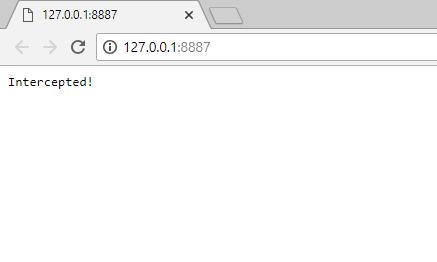
\includegraphics[width=0.7\linewidth]{Intercepted}
		\caption{Intercepted}
		\label{fig: Intercepted}
	\end{figure}
	
	\newpage
	\section{Compatibilità web}
	\subsection{Desktop}
	\begin{figure}[h]
		\centering
		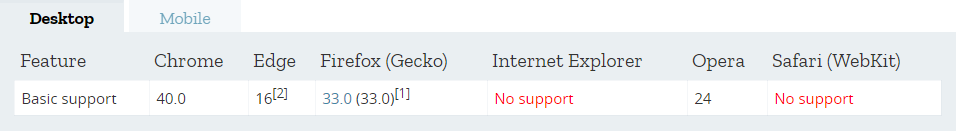
\includegraphics[width=1\linewidth]{CompWeb}
		\caption{Compatibilità web}
		\label{fig:Compatibilità web}
	\end{figure}
	\subsection{Mobile}
	\begin{figure}[h]
		\centering
		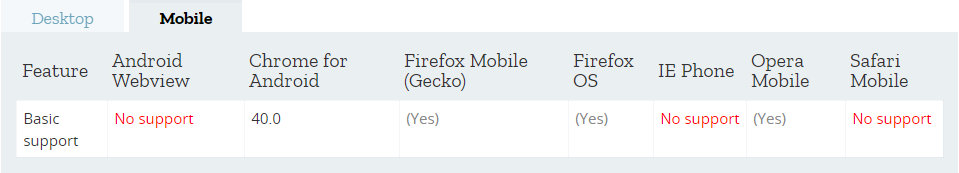
\includegraphics[width=1\linewidth]{CompMobile}
		\caption{Compatibilità mobile}
		\label{fig:Compatibilità mobile}
	\end{figure}
	\section{Conclusioni}
	Dopo questo lungo discorso si è capito che i Service Worker sono uno strumento potentissimo, e come ogni strumento possono essere usati in modo benevolo o malevolo.
	Se realizzati per fare caching possono rendere la navigazione del sito web o dell'applicazione molto veloce senza rendere necessarie modifiche al sito o all'applicazione per raggiungere tale scopo. 
	Purtroppo, come si è visto negli ultimi paragrafi, sono anche uno potente strumento a scopo malevolo.
	
	Anche qui, come nei due capitoli precedenti, abbiamo analizzato le specifiche e i problemi di privacy che tale API può avere e, come fatto in precedenza, identificheremo i vari threat model.
	Per quanto riguarda il primo caso, le migliorie dell'esperienza utente riguardono certamente il caching e la velocità con il quale le informazioni vengono caricate molto più velocemente.
	Il secondo e il terzo threat model sono simili alla Payment Request API, ovvero si tratta di vulnerabilità XSS.
	Per mitigare i rischi vi sono le direttive scritte al paragrafo precedente, ovvero il fatto che il limite di tempo di un Service Worker nella cache è di 24 ore, o meno in base alle impostazioni; in alternativa, o in aggiunta, si possono comunque usare, come nel caso delle altre API, software di sicurezza per proteggersi dai rischi all'interno del web.
	
	
	\newpage
	\cleardoublepage
	\chapter{Conclusioni}
	Questa tesi ha cercato di rispondere alla domanda: \textit{"Come faccio ad individuare i rischi di queste APIs e come posso affrontarli?"}. A tal fine è stato preso un campione di tre APIs e sono state condotte delle ricerche e degli studi per rivelare le vulnerabilità di ognuna di esse, trovandone diverse in ognuna di quelle prese in considerazione. 
	\\
	Come già detto durante tutta la tesi tali vulnerabilità possono essere colmate, o comunque evitate; chiaramente sono avantaggiate a tale riguardo le persone sempre a contatto coi mezzi tecnlogici e sicuramente anche le nuove generazioni le quali sono cresciute in mezzo alla tecnologia. Questo è un fattore  da tenere in considerazione dato che a mio parere alcuni rischi, come immettere i propri dati o consentire di rilevare la propria posizione in un sito non sicuro, sono prevalenti in certe fasce d'età. Questa considerazione si basa sulla mia esperienza personale e, per questo motivo, non è una dichiarazione generale e oggettiva. Il dato oggettivo sono i problemi legati alle diverse APIs che ho espresso nel corso della mia tesi.
	\\
	Una ricerca potrebbe essere quella di realizzare uno studio sui problemi della sicurezza in internet nelle diverse fasce d'età, concentrandosi invece che sulle vulnerabilità delle APIs su come cercare di educare più o meno tutti ai rischi del Web.
	\cleardoublepage
	\begin{center}
		\textbf{Ringraziamenti}
	\end{center}
	\begin{flushleft}
		A conclusione di questo lavoro di tesi mi sento in dovere di porre i miei più sentiti ringraziamenti alle persone che ho avuto modo di conoscere in questo importante periodo della mia vita e che mi hanno aiutato a crescere dal punto di vista professionale ma soprattutto umano.
		\\
		Un sincero ringraziamento al mio relatore Dott. Stefano Calzavara che, oltre alla sua vastissima e precisa conoscenza nel campo della sicurezza, mi ha saputo risolvere ogni dubbio, e sopratutto mi ha aiutato a non lasciare stare questo lavoro quando la rassegnazione stava prendendo il sopravvento.
		\\
		Un grazie anche al mio correlatore Dott. Marco Squarcina che ha saputo darmi consigli fondamentali per riuscire ad andare avanti in alcuni punti della tesi che altrimenti non avrei saputo risolvere da solo.
		\\
		Non possono mancare in questo elenco tutti i miei compagni di corso con i quali ho trascorso questi anni nelle aule dell'università tra risate, scene uniche e indimenticabili e terrore durante qualche esame, con i quali ho instaurato un rapporto di amicizia che spero duri nel tempo.
		\\
		Una dose importante di ringraziamenti va a tutti quei miei amici che, dicendomi la giusta dose di parole nei momenti opportuni ma aiutandomi altrettante volte e soprattutto spendendo gran parte del loro tempo per darmi una mano, sono riuscite a farmi compiere questo percorso. Grazie davvero.
		\\
		Dovrei scrivere un'altra tesi se scrivessi ad una ad una tutte le persone che, in diverse forme, mi hanno aiutato a superare tutti i problemi e i brutti periodi di questi anni universitari. Sicuramente uno dei motivi per cui sono arrivato fino a qua è stato anche grazie al continuo "Ce la fai, non mollare!" in risposta ai miei "Lascio stare tutto, non sono capace". 
		\\
		Per ultimi, ma non meno importanti, i miei genitori.
		Non so se troverò mai le parole giuste per ringraziarvi, però vorrei che questo traguardo ripagasse, per quanto possibile, tutti i sacrifici che hanno fatto per me, e che fosse un premio anche per loro.
		Un grande grazie a tutta la mia famiglia per esserci sempre, per sostenermi in ogni cosa io faccia, e sicuramente senza i vostri consigli e le vostre critiche non sarei la persona che sono oggi.
		Grazie per avermi fatto arrivare a questo punto di arrivo e contemporaneamente di partenza della mia vita.
	\end{flushleft}
\cleardoublepage
\listoffigures
\cleardoublepage
	%\section{Sitografia}	
	
	\bibliography{Referenze}
\end{document}